\section{Motivation}

\begin{frame}
	{Motivation}	
	{Image analysis}

\begin{minipage}[t][0.5\textheight][t]{1\textwidth}
The problems we are interested in come from \emph{image analysis}.
\vspace{1em}

\only<1-4>{
\begin{center}
\begin{tabular}{ccc}
\highlight{2}{1,3-}{\textbf{Segmentation}} & 
\highlight{3}{1-2,4-}{\textbf{Denoising}} & 
\highlight{4}{1-3,5-}{\textbf{Inpainting}}
\end{tabular}
\end{center}}

\only<2>{
\center
\begin{tabular}{p{0.4\textwidth}c}
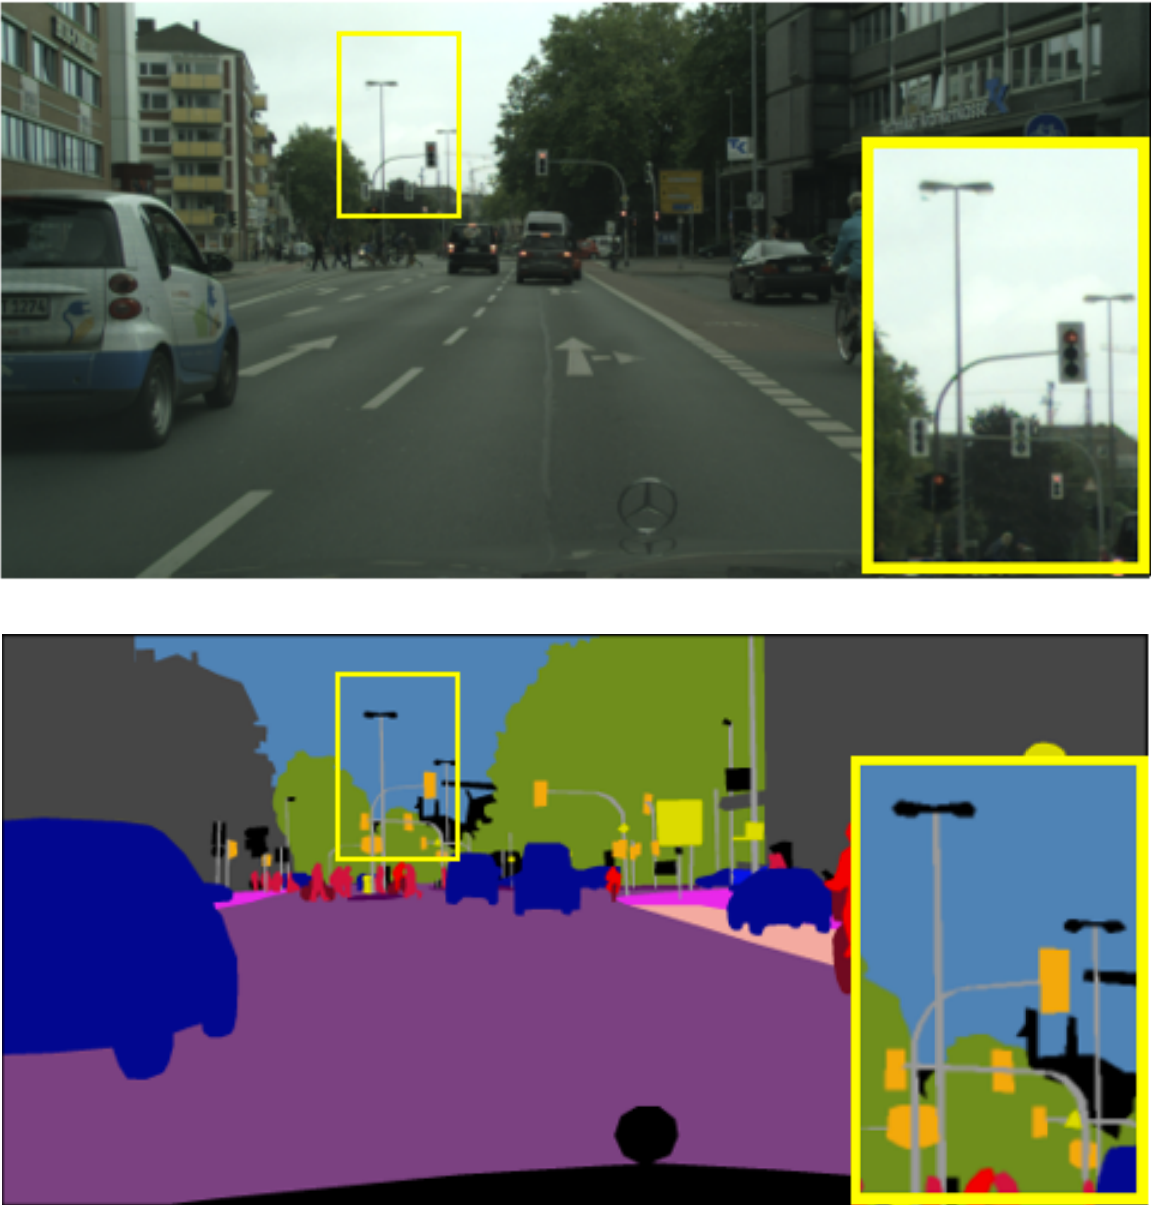
\includegraphics[scale=0.4]{figures/motivation/image-analysis/segmentation-cars.png} &
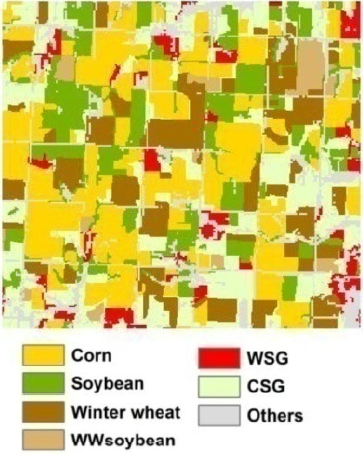
\includegraphics[scale=0.4]{figures/motivation/image-analysis/segmentation-crops.png}\\
\mycite{li2019gff} & \mycite{li2015object}
\end{tabular}}%
\only<3>{
\center
\begin{tabular}{cc}
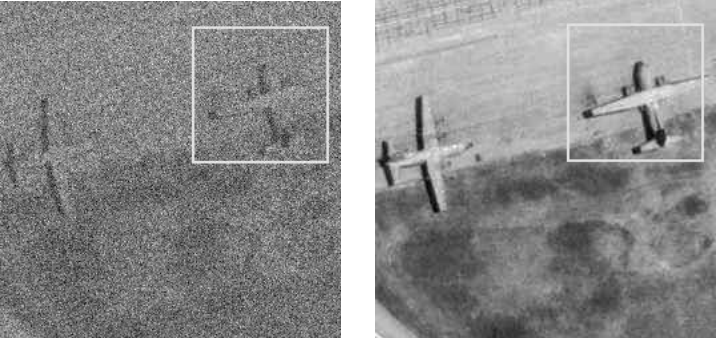
\includegraphics[scale=0.44]{figures/motivation/image-analysis/denoising-airplane.png} &
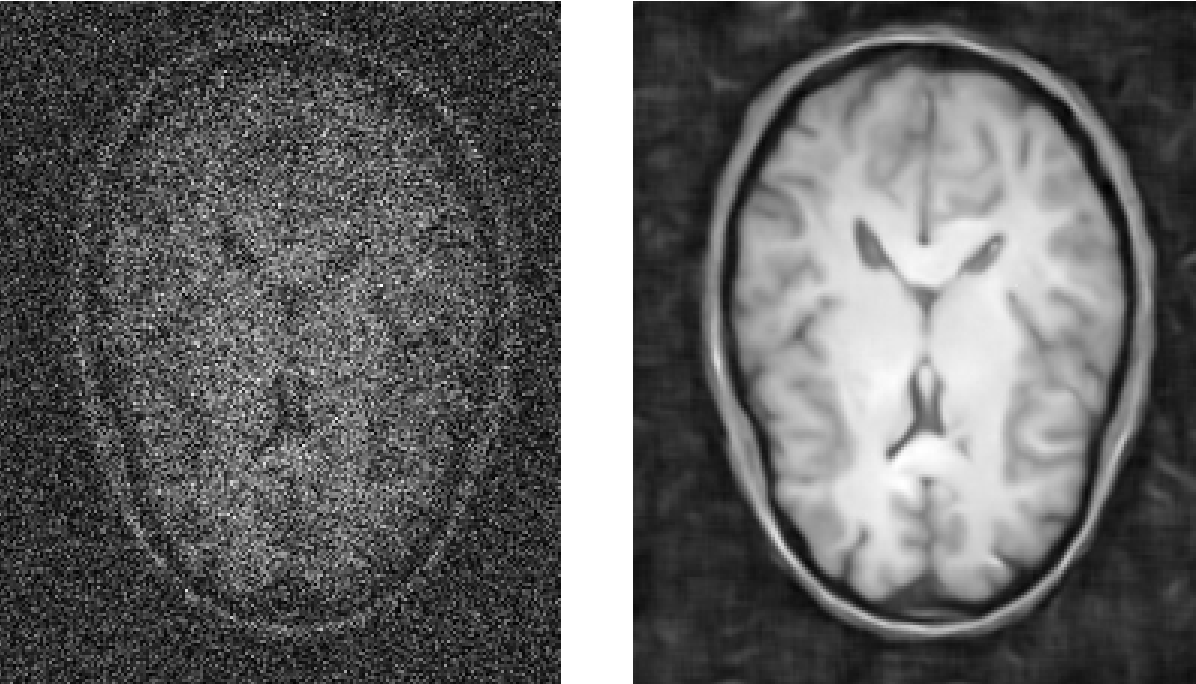
\includegraphics[scale=0.22]{figures/motivation/image-analysis/denoising-mri.png} \\
\mycite{xu2018deep} & \mycite{jiang2018denoising}
\end{tabular}}%
\only<4>{
\center
\begin{tabular}{cc}
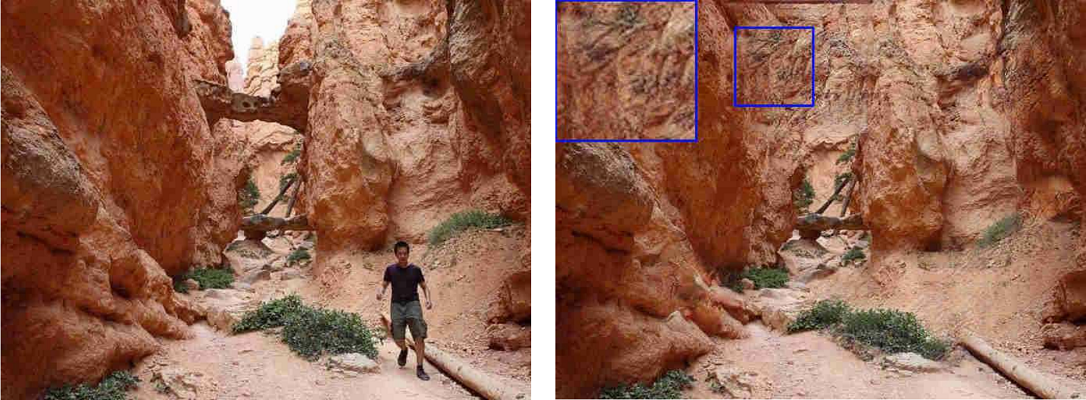
\includegraphics[scale=0.3]{figures/motivation/image-analysis/inpainting-man.png} &
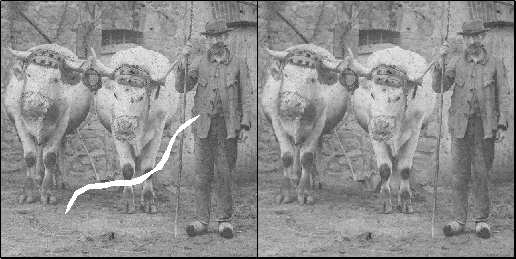
\includegraphics[scale=0.24]{figures/motivation/image-analysis/inpainting-picture.png} \\
\mycite{yu2018generative} &  \mycite{masnou98inpainting}
\end{tabular}}%
\only<5->{
\begin{tabular}{p{0.6\textwidth}p{0.2\textwidth}}
\textbf{Segmentation:} $\mathcal{I}^{\star} = \argmin_{\mathcal{I}} E_{seg}(\mathcal{I},f_{\vec{I}}).$ & \raisebox{-.5\height}{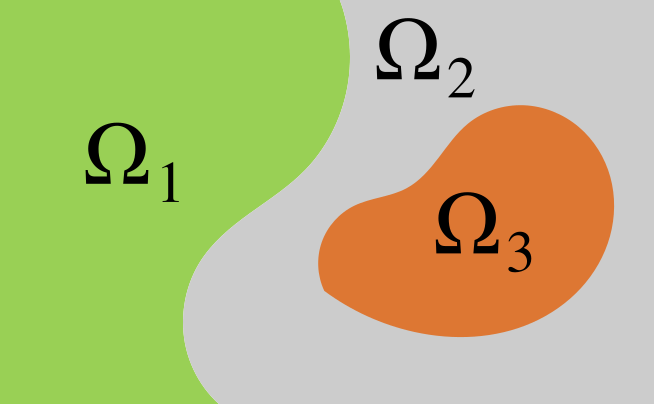
\includegraphics[scale=0.24]{figures/motivation/image-analysis/segmentation-stylised.png}}\\[2em]
\textbf{Denoising:} $f_{\widehat{\vec{I}}} = \argmin_f E_{den}(f,f_{\vec{\widetilde{I}}}).$ & \raisebox{-.5\height}{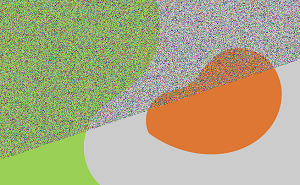
\includegraphics[scale=0.24]{figures/motivation/image-analysis/denoising-stylised.png}}\\[2em]
\textbf{Inpainting:} $f_{\vec{\widehat{I}}} = \argmin_f E_{inp}(f,f_{\widetilde{\vec{I}}}).$ & \raisebox{-.5\height}{
\includegraphics[scale=0.24]{figures/motivation/image-analysis/inpainting-stylised.png}}
\end{tabular}}
\end{minipage}
%6
%
\begin{minipage}[t][0.27\textheight][t]{\textwidth}
\only<5->{We focused on \emph{variational approaches} to solve these problems.}

\only<6->{
Energies are defined by terms that guides the optimization towards solution of interest, e.g.,
\begin{itemize}
	\item{ \emph{Data fidelity}. The solution should not differ much from the input. }
	\item{ \emph{Spatial coherence}. Images are composed of regions with low variability in color. }
\end{itemize}
}
\end{minipage}

\end{frame}







\begin{frame}
{Motivation}
{Geometric priors}
The \emph{Mumford Shah}~(\mycite{mumford89}) is a model for segmentation and denoising.
%
%
\begin{align*}
	\min_{f,\highlight{4}{1-3,5-}{\mathcal{K}}} \alpha \int_{\Omega} \highlight{2}{1,3-}{\norm{ f_{\vec{I}} - f}^2}dx + \beta \int_{\Omega \setminus \highlight{4}{1-3,5-}{\mathcal{K}}} \highlight{3}{1,2,4-}{\norm{ \nabla f}^2} dx + \lambda Per(\highlight{4}{1-3,5-}{\mathcal{K}}).
\end{align*}
%
%
\onslide<5->{
The \emph{ROF}~(\mycite{rudin92}) model uses \emph{total variation} for image denoising.
%
%
\begin{align*}
	\min_{f} \alpha \int_{\Omega} \norm{ f_{\vec{I}} - f}^2dx + \beta \int_{\Omega} \highlight{6}{1-5,7-}{\norm{ \nabla f }}dx.
\end{align*}}
%
%
\onslide<7->{
\begin{itemize}
	\item{A measure of perimeter is present in both models.}
	\item{\emph{Geometric priors} as perimeter, area or curvature are useful due to their flexibility and predictability.}
\end{itemize}}
%
%
\vspace{1em}
\onslide<8->{
In this thesis, we are interested in the combined use of \emph{perimeter} and \emph{squared curvature} as geometric priors.}
\end{frame}

\begin{frame}
{Motivation}
{Completion property}
\begin{minipage}[t][0.5\textheight][t]{\textwidth}
\only<1->{
\center
$\min_{ X \subset \Omega } Data(X) + Perimeter(\partial X).$
}
\only<1>{
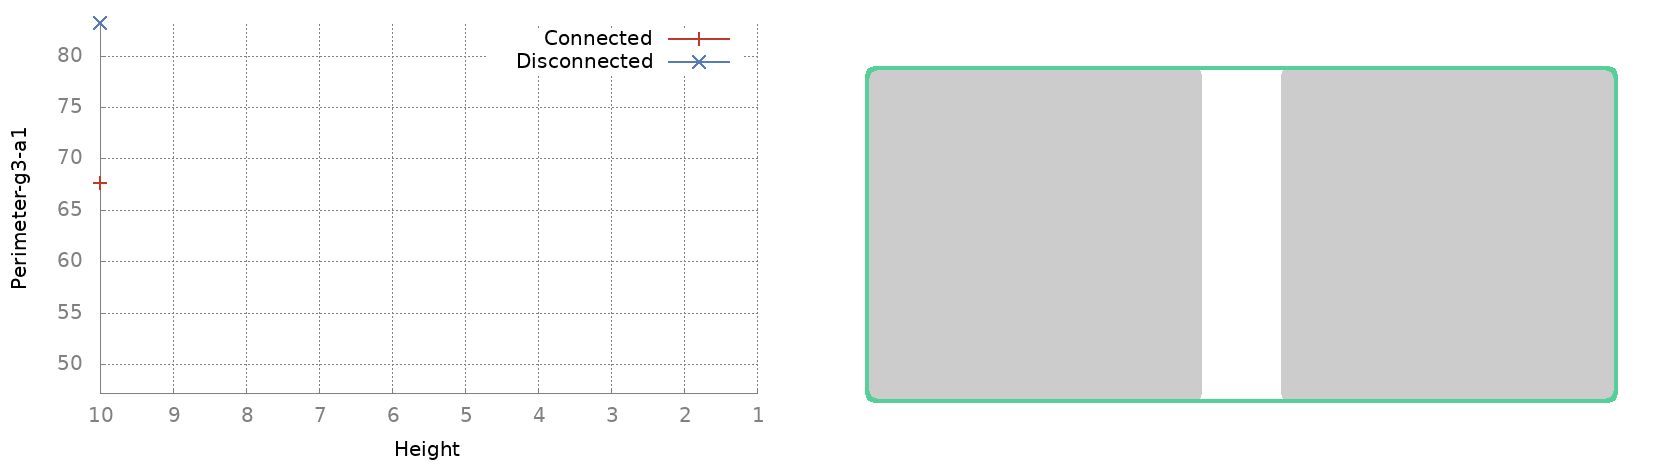
\includegraphics[scale=0.25]{figures/motivation/completion/perimeter-0.png}
}
\only<2>{
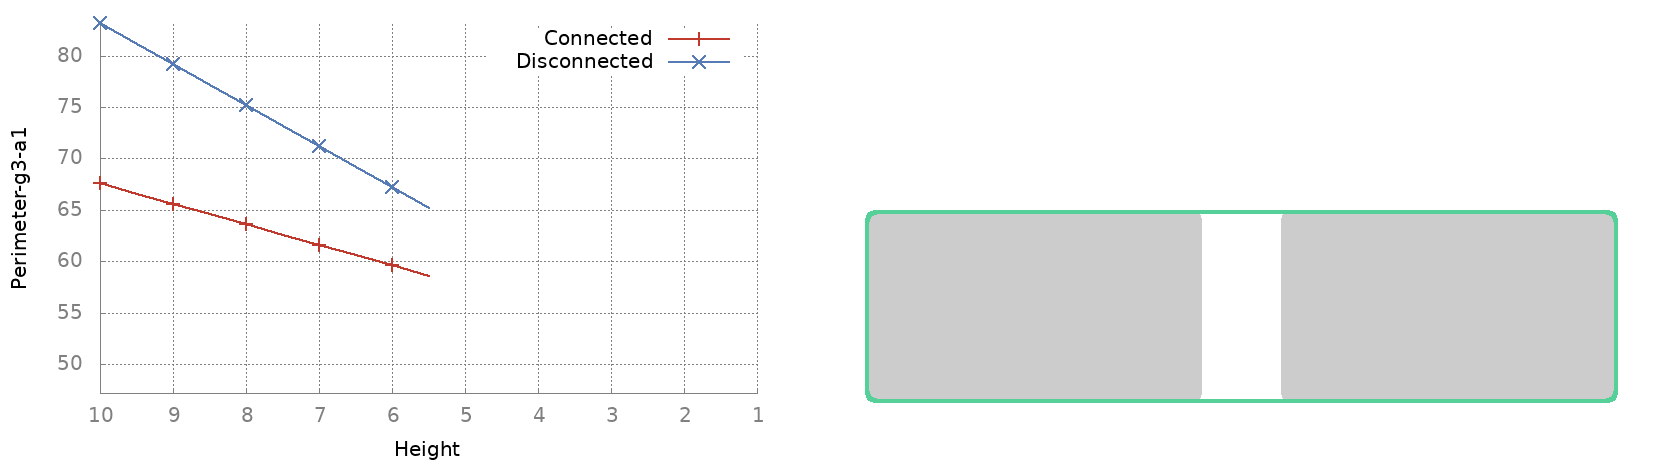
\includegraphics[scale=0.25]{figures/motivation/completion/perimeter-1.png}
}
\only<3>{
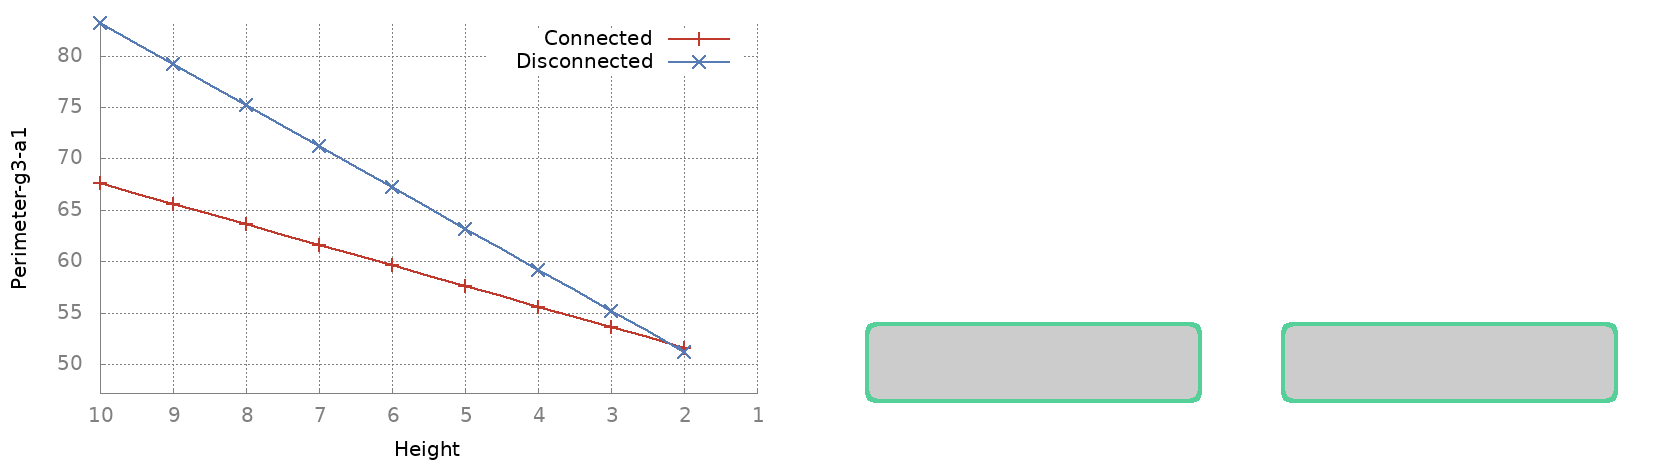
\includegraphics[scale=0.25]{figures/motivation/completion/perimeter-2.png}
}
\only<4->{
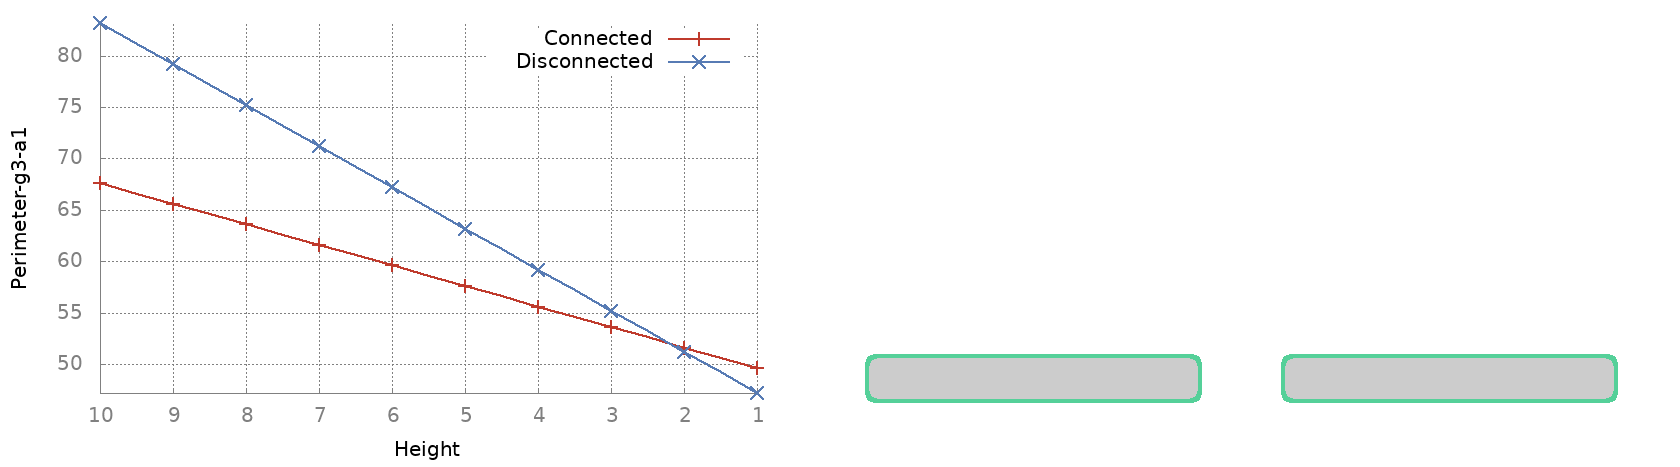
\includegraphics[scale=0.25]{figures/motivation/completion/perimeter-3.png}
}
\end{minipage}
\begin{minipage}[t][0.5\textheight][t]{\textwidth}
\only<5->{
\center
$\min_{ X \subset \Omega } Data(X) + Perimeter(\partial X) + Curvature^2(\partial X).$}
\only<5>{
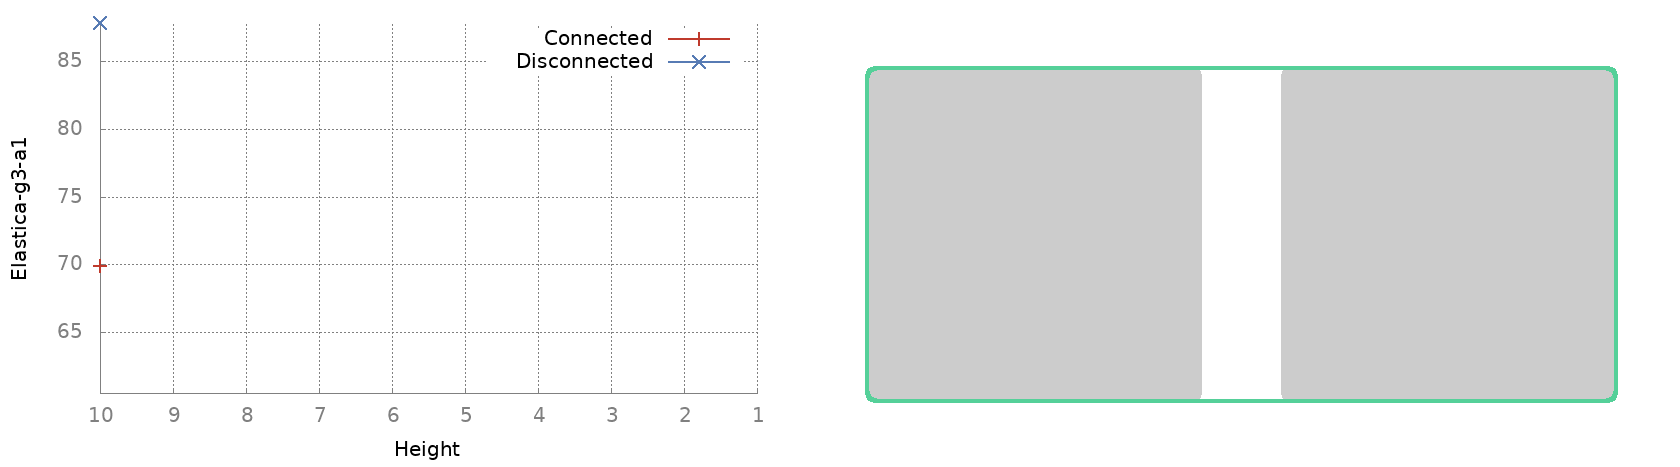
\includegraphics[scale=0.25]{figures/motivation/completion/elastica-0.png}
}
\only<6>{
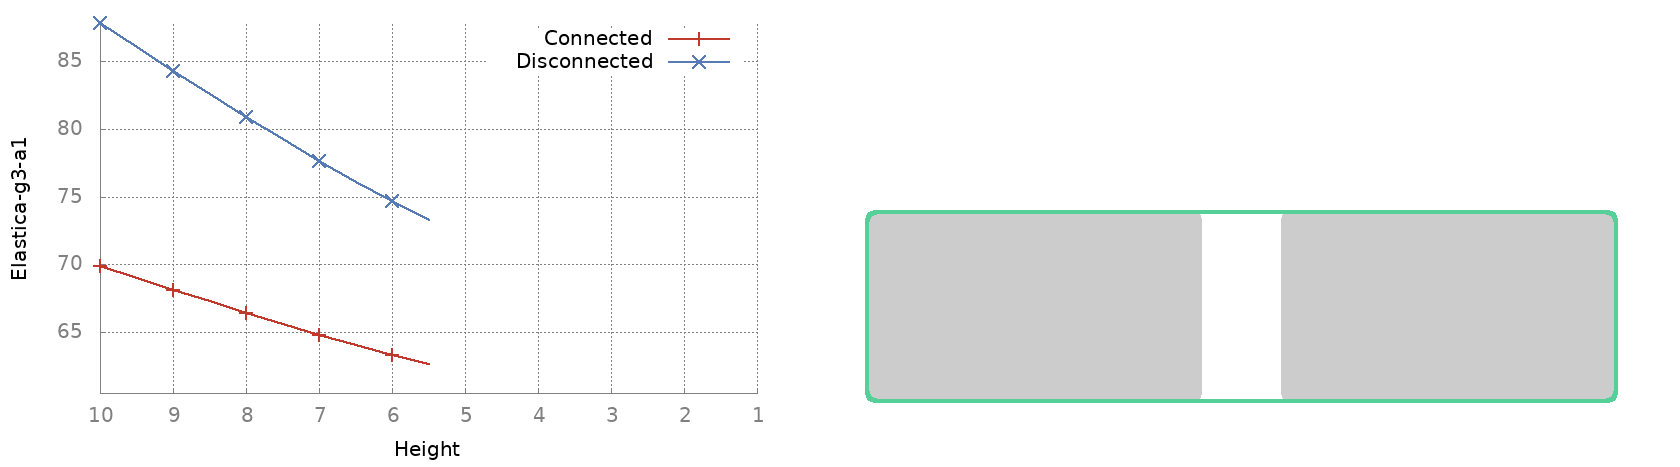
\includegraphics[scale=0.25]{figures/motivation/completion/elastica-1.png}
}
\only<7>{
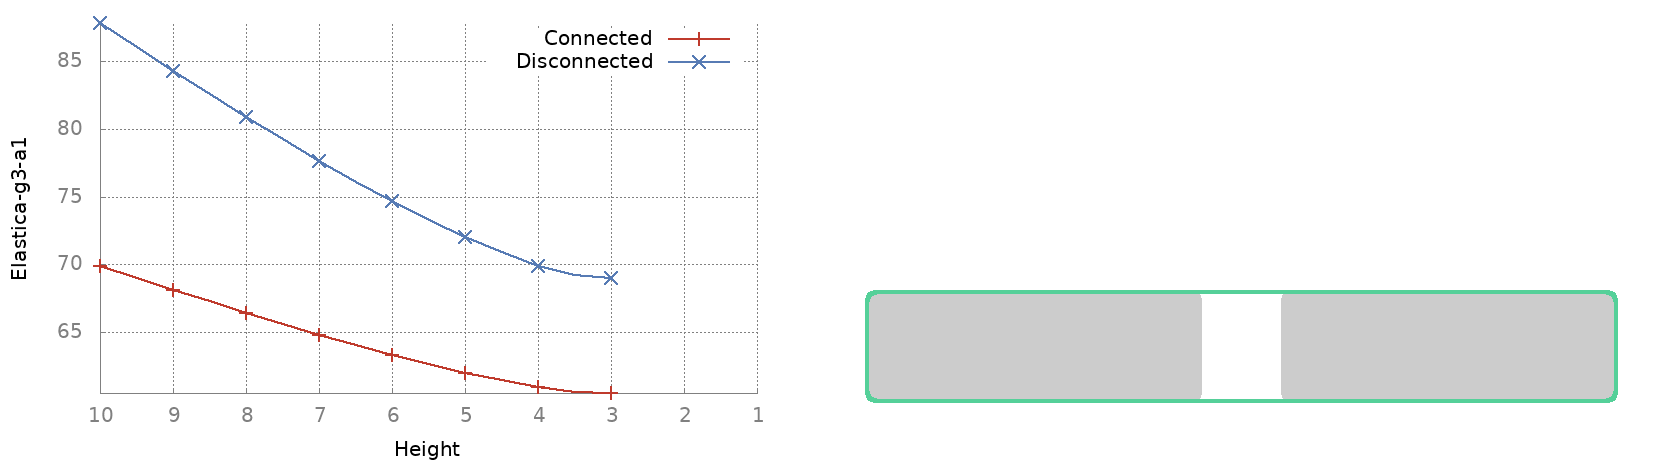
\includegraphics[scale=0.25]{figures/motivation/completion/elastica-2.png}
}
\only<8->{
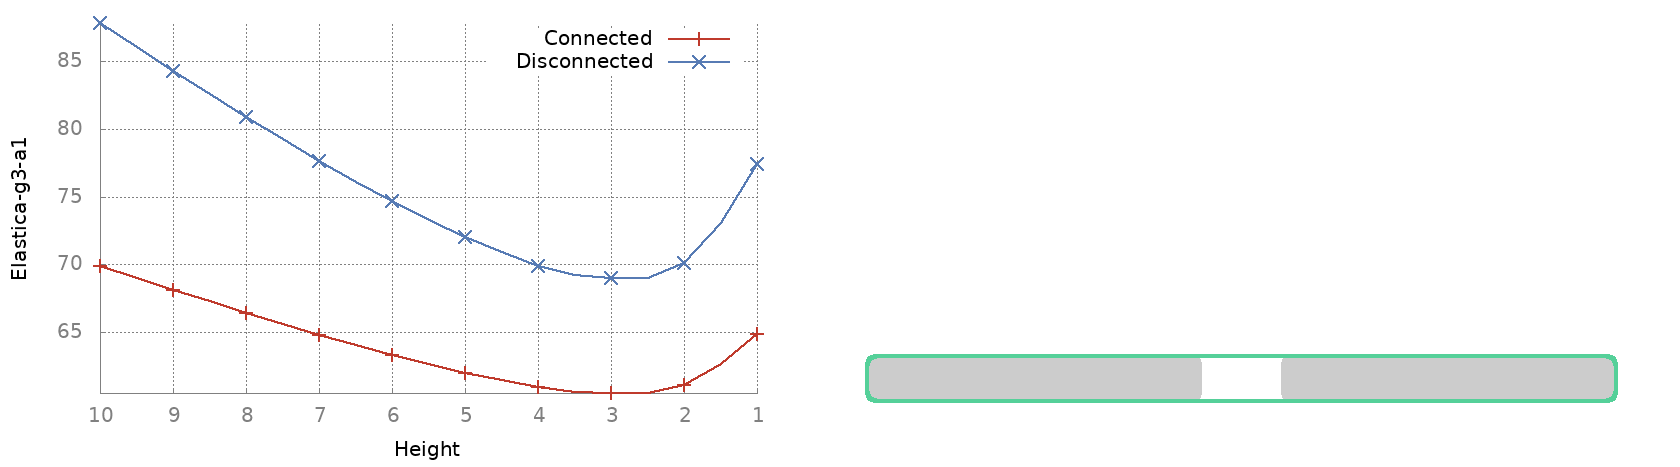
\includegraphics[scale=0.25]{figures/motivation/completion/elastica-3.png}
}
\end{minipage}
\end{frame}

\begin{frame}
{Motivation}
{Completion property}
\begin{minipage}[t][0.5\textheight][t]{\textwidth}
\only<1->{
\center
$\min_{ X \subset \Omega } Data(X) + Perimeter(\partial X) + Curvature^2(\partial X).$}
\only<1>{
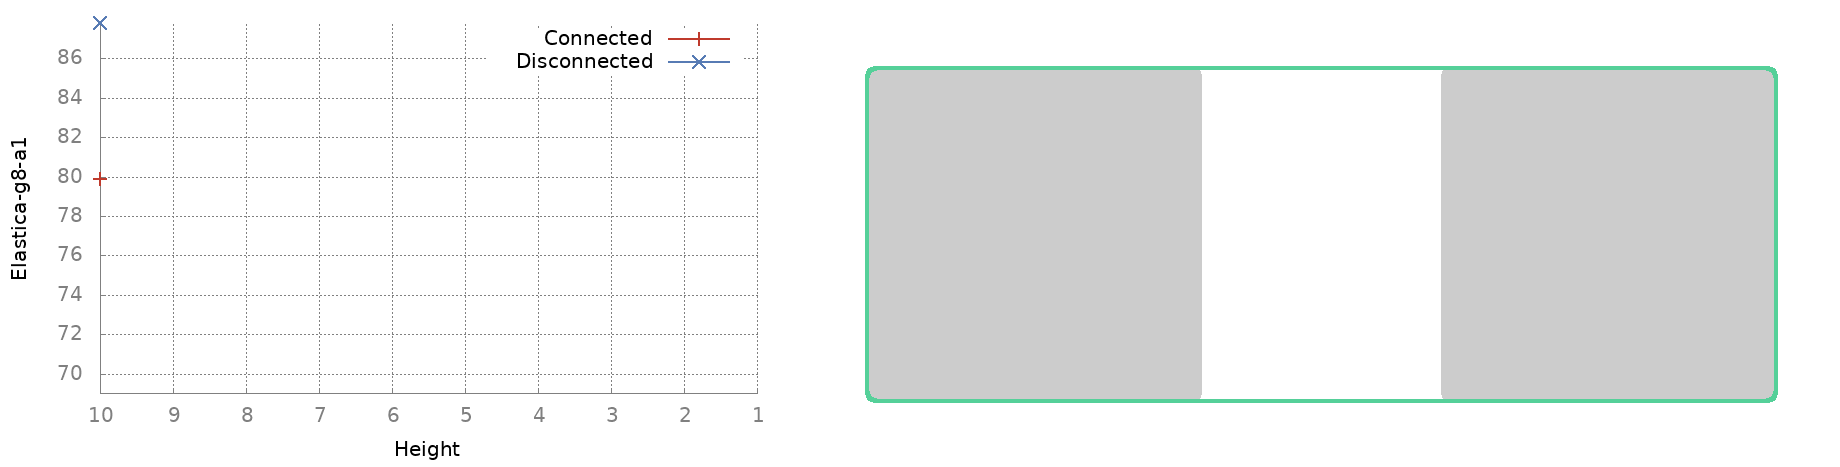
\includegraphics[scale=0.22]{figures/motivation/completion/elastica-g8a1-0.png}
}%
\only<2>{
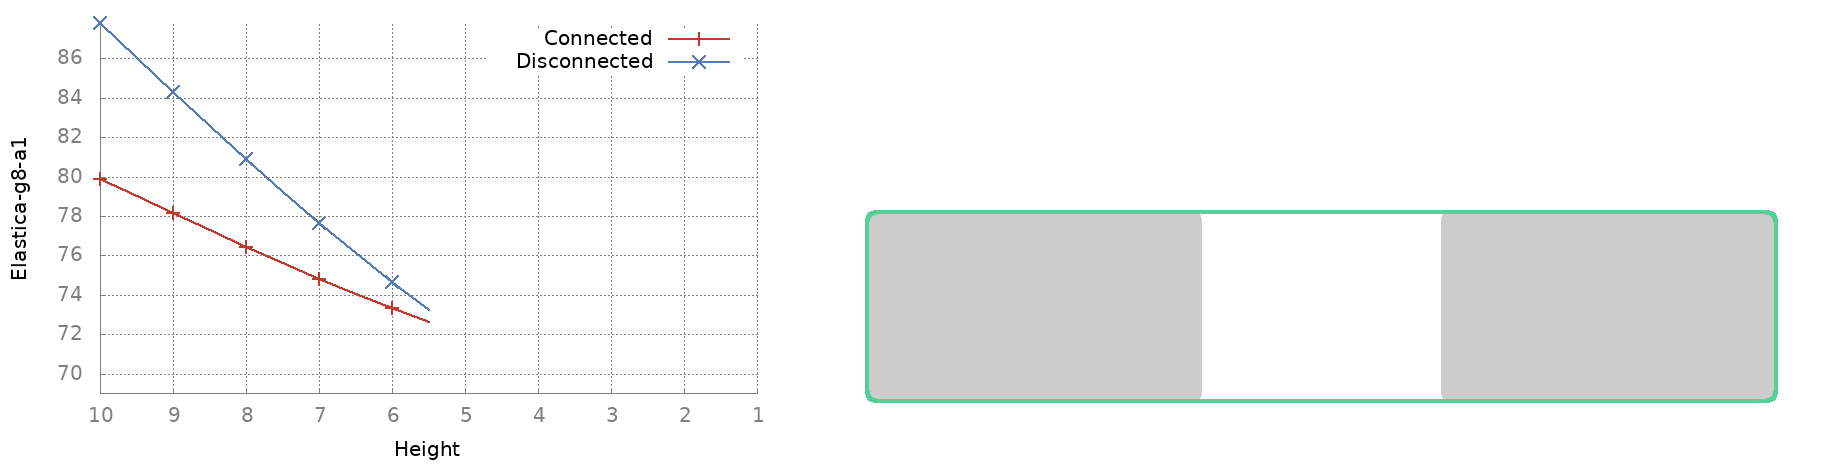
\includegraphics[scale=0.22]{figures/motivation/completion/elastica-g8a1-1.png}
}%
\only<3>{
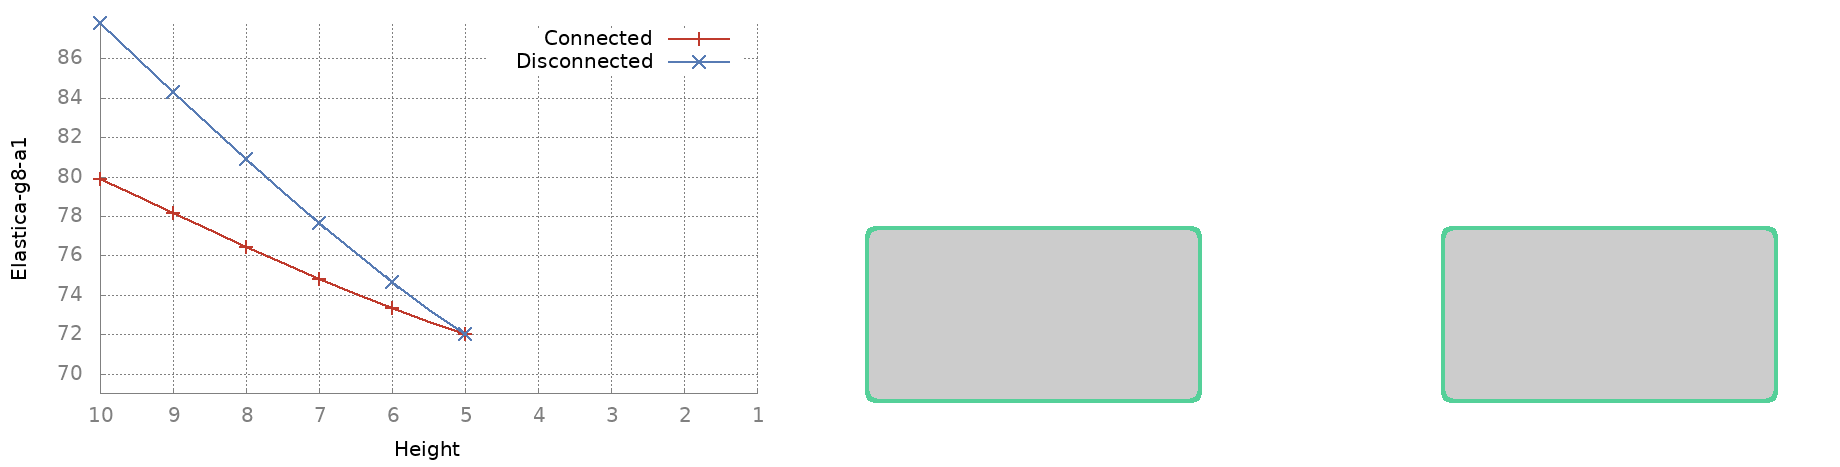
\includegraphics[scale=0.22]{figures/motivation/completion/elastica-g8a1-2.png}
}%
\only<4>{
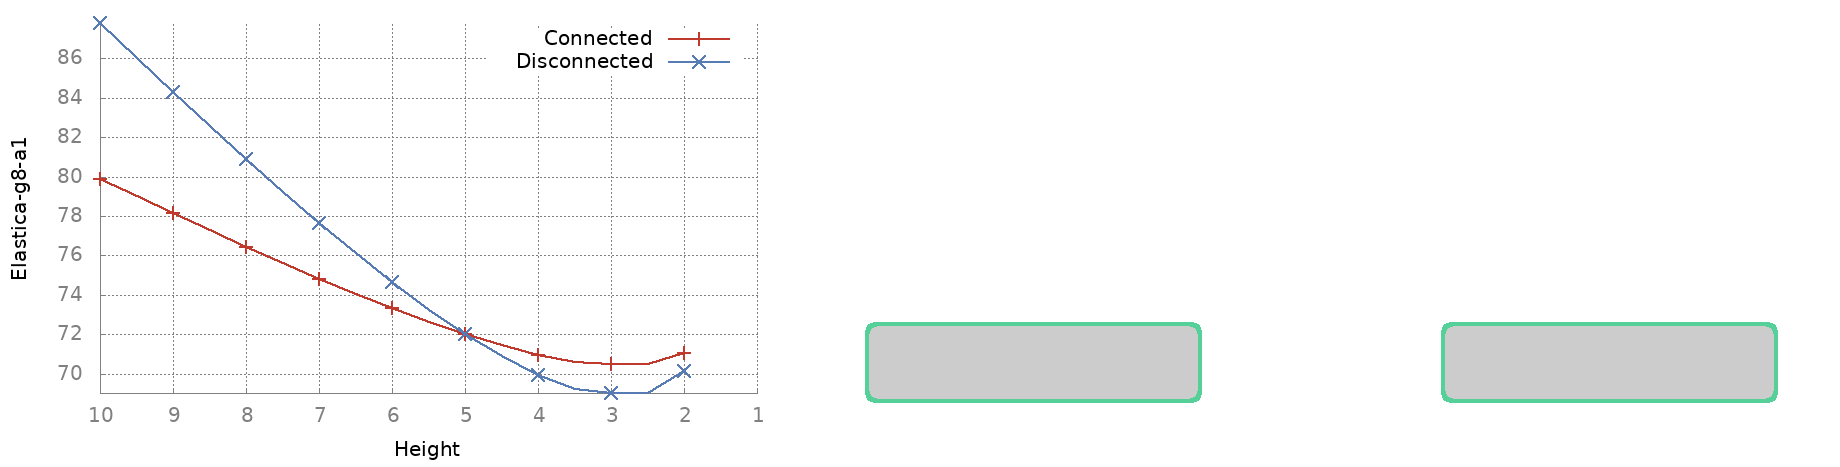
\includegraphics[scale=0.22]{figures/motivation/completion/elastica-g8a1-3.png}
}%
\only<5->{
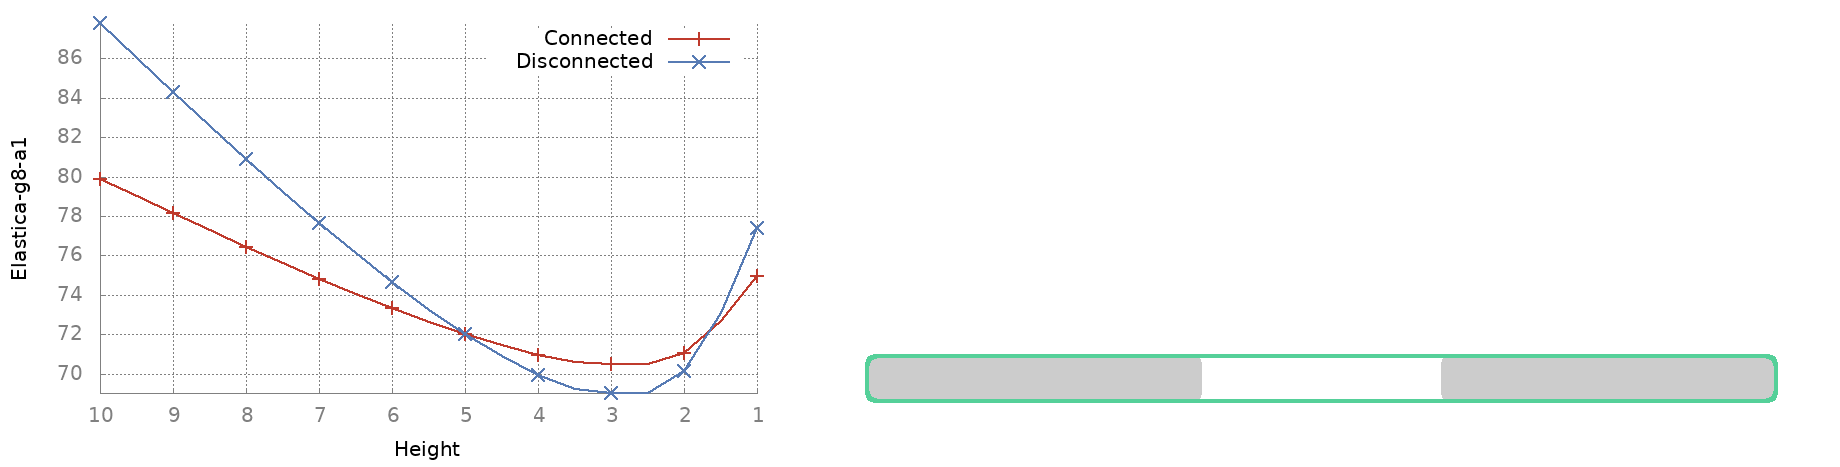
\includegraphics[scale=0.22]{figures/motivation/completion/elastica-g8a1-4.png}
}%
%
\begin{tikzpicture}
    \node at (current page.north east)
        {%
        \begin{tikzpicture}[remember picture, overlay]
		\draw [xshift=0.6cm,yshift=1.2cm,decorate,decoration={brace,amplitude=5pt,mirror,raise=4ex}]
		  (1,0) -- (2.5,0) node[midway,yshift=-3em]{Larger gap};
	  \end{tikzpicture}
	  };%
\end{tikzpicture}
%
\end{minipage}
\begin{minipage}[t][0.5\textheight][t]{\textwidth}
\only<6-9>{
\center
$\min_{ X \subset \Omega } Data(X) + {\color{highlightcolor} \frac{1}{2}} Perimeter(\partial X) + Curvature^2(\partial X).$}
\only<10->{
\center
\color{highlightcolor} $\min_{ X \in \Omega } \int_{\partial X}{ \alpha + \beta \kappa ^2ds}. \quad - \quad \text{The elastica energy}$}
\only<6>{
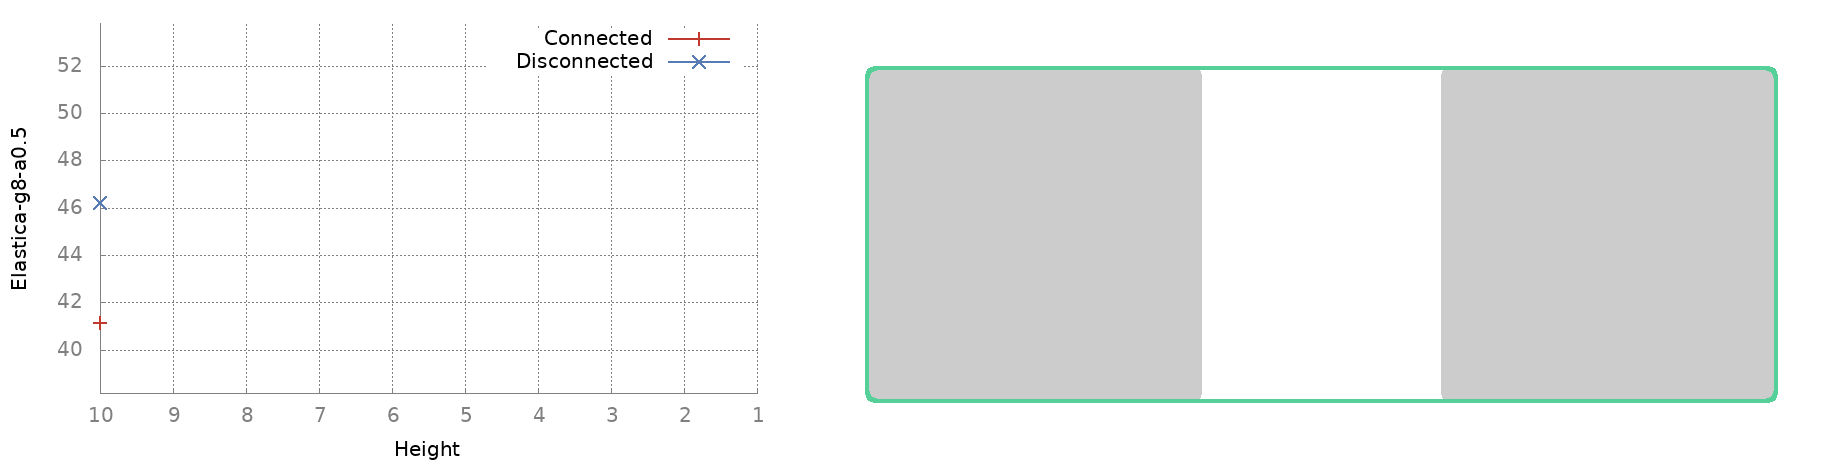
\includegraphics[scale=0.22]{figures/motivation/completion/elastica-g8a05-0.png}
}
\only<7>{
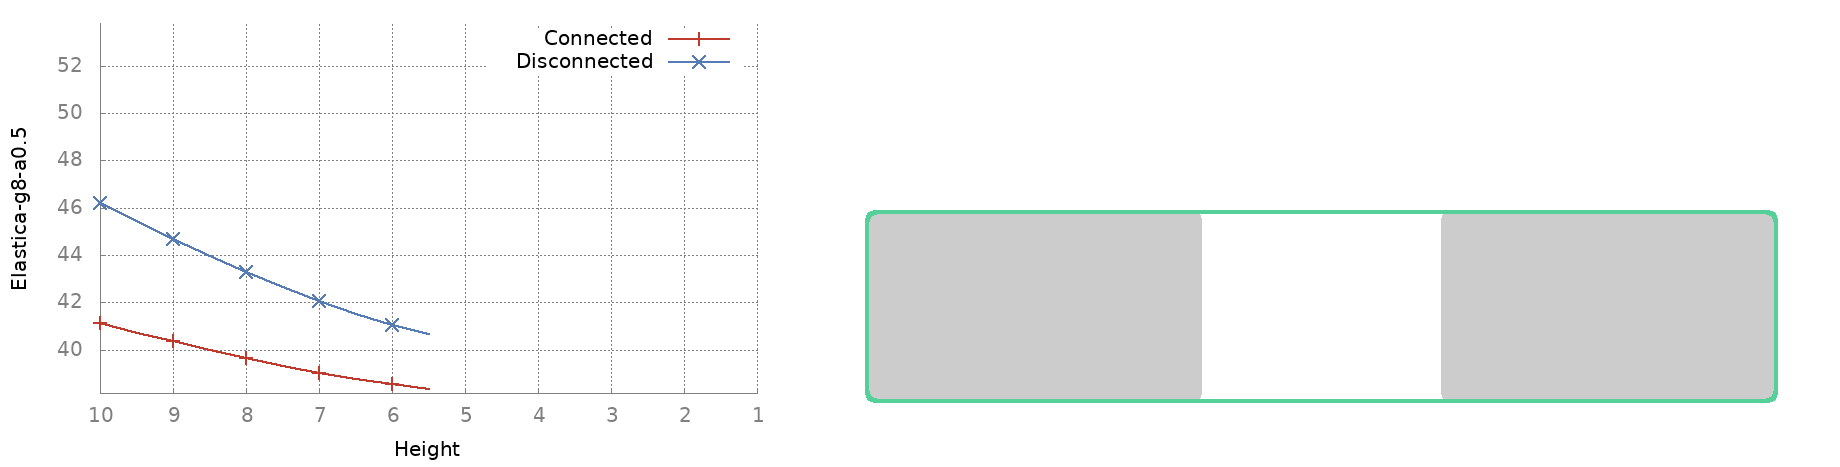
\includegraphics[scale=0.22]{figures/motivation/completion/elastica-g8a05-1.png}
}
\only<8>{
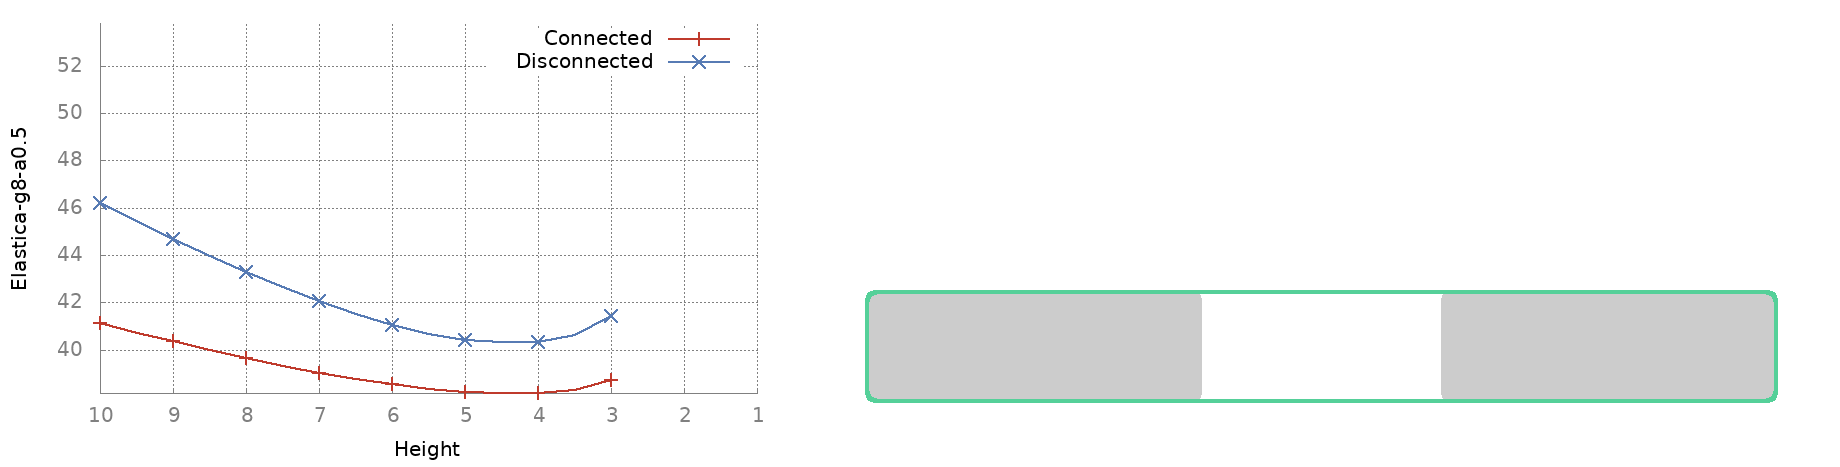
\includegraphics[scale=0.22]{figures/motivation/completion/elastica-g8a05-2.png}
}
\only<9->{
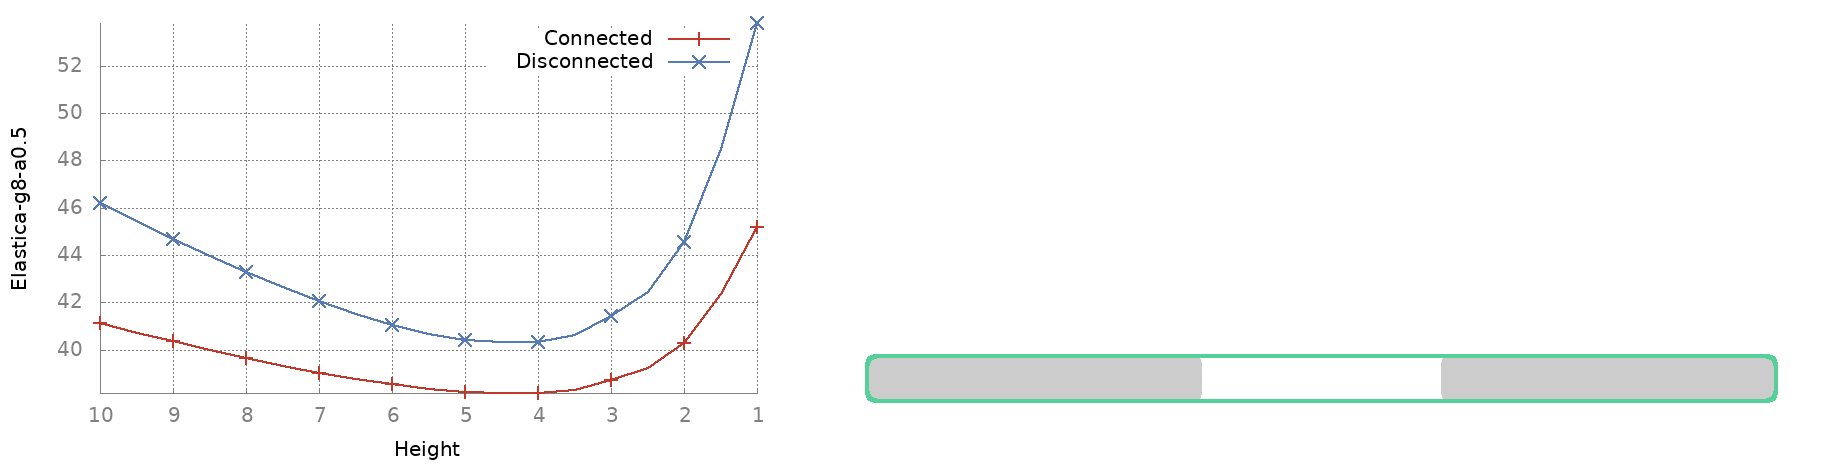
\includegraphics[scale=0.22]{figures/motivation/completion/elastica-g8a05-3.png}
}
\onslide<11>{
	\begin{figure}
	\begin{tikzpicture}[overlay, remember picture] 
	\node at (current page.center) 
	    [
	    anchor=east,
	    xshift=-10mm,
	    yshift=0mm
	    ] 
	{
	
	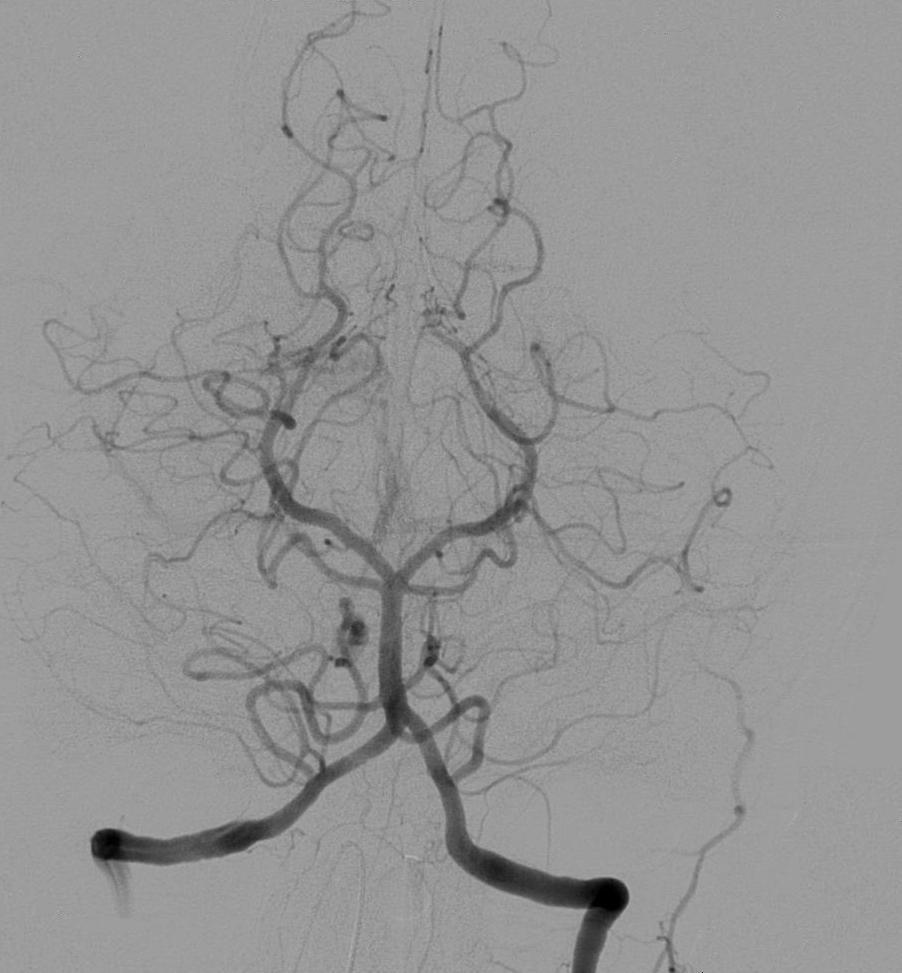
\includegraphics[scale=0.16]{figures/motivation/completion/angiogram.jpg}
		
	};
	\node at (current page.center) 
	    [
	    anchor=west,
	    xshift=-10mm,
	    yshift=0mm
	    ] 
	{
	
	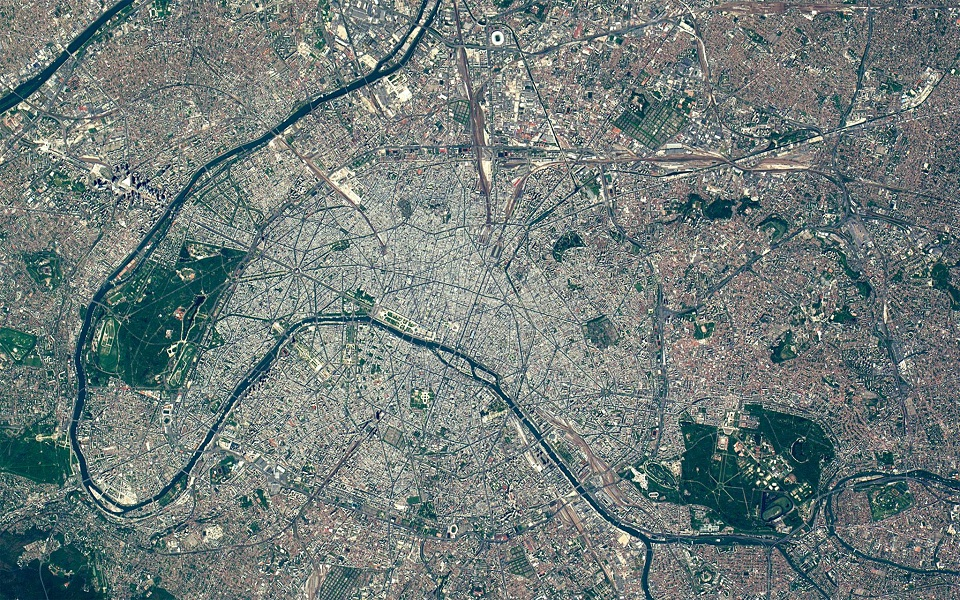
\includegraphics[scale=0.35]{figures/motivation/completion/paris-satellite-road.jpg}
		
	};	
	\end{tikzpicture}	
	\end{figure}	
	}	
\end{minipage}
\end{frame}

\begin{frame}
{Motivation}
{State-of-the-art}
\small
\textbf{Continuous setting}: Define the energy over the whole domain and minimize the elastica with respect the level-curves~(\mycite{chan02elasticainpainting}).
%
\begin{align*}
\int_{\Omega}{ \left(\alpha + \beta \nabla \cdot \left(\frac{\nabla f_{\vec{I}}}{\norm{\nabla f_{\vec{I}} }}\right) ^2 \right)\norm{\nabla f_{\vec{I}} }d\Omega}.
\end{align*}
%
\pause
\begin{itemize}
\item{Numerical instability: Fourth-order Euler-Lagrange equation.}
\item{Susceptible to bad local minimum.}
\end{itemize}
%
\pause
\vspace{0.5em}
\textbf{Discrete setting}:
\vspace{-1em}
\setlength\tabcolsep{3pt}
\begin{center}
\renewcommand{\arraystretch}{0.25}
\begin{tabular}{p{0.4\textwidth}p{0.6\textwidth}}
T-junctions matching & \multirow{2}{0.6\textwidth}{\footnotesize Fast algorithm, but limited to absolute value of curvature (polygonal solutions) and inpainting application.} \\
\mycite{masnou98inpainting} &\pause\\[3em]
Linear programming & \multirow{2}{0.6\textwidth}{\footnotesize Global formulation, but prohibitive running times even for small (thus unprecise) neighborhoods. Not suitable for digital sets.} \\
\mycite{schoenemann09linear} &\pause\\[3em]
Triple cliques & \multirow{2}{0.6\textwidth}{\footnotesize Global formulation, quadratic non-submodular energy. Limited precision due combinatorial explosion.} \\
\mycite{nieuwenhuis14efficient} &
\end{tabular}
\end{center}
\end{frame}

\begin{frame}
{Motivation}
{Goals}

Models based on the minimization of the elastica energy

\center
\begin{tabular}{lcc|c|}
& Continuous & Discrete & \textbf{Digital} \\
\hline
Numerical instability & \negative{Yes} & \positive{No} & \positive{No} \\
Suitable for digital sets & \negative{No} & \negative{No} & \positive{Yes} \\
Rounding issues & \negative{Yes} & \positive{No} & \positive{No} \\
Contour completion & \negative{Partial} & \negative{Partial} & \positive{Extended} \\
Global formulation & \positive{Yes} & \positive{Yes} & \negative{No} \\
Global optimum (Free elastica) & \negative{-} & \negative{-} & \positive{Yes}
\end{tabular}

%\vspace{2em}
%
%\begin{itemize}
%\item{Can we define an elastica-based model for image analysis using multigrid convergent estimators? \only<4>{\positive{Yes!}}} \pause
%\item{Can we recover the completion property of elastica? \only<4>{\positive{Yes!}}} \pause
%\item{Can we escape bad local minima? \only<4>{\positive{Yes!}}}
%\end{itemize}

\end{frame}

